\documentclass[journal,12pt,twocolumn]{IEEEtran}
%
\makeatletter
\makeatother
\usepackage{setspace}
\usepackage{gensymb}
\usepackage{xcolor}
\usepackage{caption}
%\usepackage{stackengine}
%\usepackage{subcaption}
%\doublespacing
\singlespacing

\usepackage{pgf}
\usepackage{tikz}
\usetikzlibrary{arrows,automata}
\usepackage[latin1]{inputenc}


\usepackage{graphicx}
%\graphicspath{ {./images}  }
%\usepackage{amssymb}
%\usepackage{relsize}
\usepackage[cmex10]{amsmath}
\usepackage{mathtools}
%\usepackage{amsthm}
%\interdisplaylinepenalty=2500
%\savesymbol{iint}
%\usepackage{txfonts}
%\restoresymbol{TXF}{iint}
\usepackage{wasysym}
\usepackage{amsthm}
\usepackage{mathrsfs}
\usepackage{txfonts}
\usepackage{stfloats}
\usepackage{cite}
\usepackage{cases}
\usepackage{mathtools}
\usepackage{subfig}
\usepackage{enumerate}	
\usepackage{enumitem}
\usepackage{amsmath}
%\usepackage{xtab}
\usepackage{longtable}
\usepackage{multirow}
%\usepackage{algorithm}
%\usepackage{algpseudocode}
\usepackage{enumitem}
\usepackage{mathtools}
%\usepackage{iithtlc}
%\usepackage[framemethod=tikz]{mdframed}
\usepackage{listings}
\usepackage{listings}
    \usepackage[latin1]{inputenc}                                 %%
    \usepackage{color}                                            %%
    \usepackage{array}                                            %%
    \usepackage{longtable}                                        %%
    \usepackage{calc}                                             %%
    \usepackage{multirow}                                         %%
    \usepackage{hhline}                                           %%
    \usepackage{ifthen}                                           %%
  %optionally (for landscape tables embedded in another document): %%
    \usepackage{lscape}     



%\usepackage{stmaryrd}


%\usepackage{wasysym}
%\newcounter{MYtempeqncnt}
\DeclareMathOperator*{\Res}{Res}
%\renewcommand{\baselinestretch}{4}
%\setcounter{secnumdepth}{4}
\renewcommand\thesection{\arabic{section}}
\renewcommand\thesubsection{\thesection.\arabic{subsection}}
\renewcommand\thesubsubsection{\thesubsection.\arabic{subsubsection}}
%\renewcommand\thesubsubsubsection{\thesubsubsection.\arabic{subsubsubsection}}

%\renewcommand\thesectiondis{\arabic{section}}
%\renewcommand\thesubsectiondis{\thesectiondis.\arabic{subsection}}
%\renewcommand\thesubsubsectiondis{\thesubsectiondis.\arabic{subsubsection}}
%\renewcommand\thesubsubsubsectiondis{\thesubsubsectiondis.\arabic{subsubsubsection}}
% correct bad hyphenation here
\hyphenation{op-tical net-works semi-conduc-tor}

%\lstset{
%language=C,
%frame=single, 
%breaklines=true
%}

%\lstset{
	%%basicstyle=\small\ttfamily\bfseries,
	%%numberstyle=\small\ttfamily,
	%language=Octave,
	%backgroundcolor=\color{white},
	%%frame=single,
	%%keywordstyle=\bfseries,
	%%breaklines=true,
	%%showstringspaces=false,
	%%xleftmargin=-10mm,
	%%aboveskip=-1mm,
	%%belowskip=0mm
%}

%\surroundwithmdframed[width=\columnwidth]{lstlisting}
\def\inputGnumericTable{}                                 %%

\lstset{
%language=python,
frame=single, 
breaklines=true,
columns=fullflexible
}

 

\begin{document}
%

\theoremstyle{definition}
\newtheorem{theorem}{Theorem}[section]
\newtheorem{problem}{Problem}
\newtheorem{proposition}{Proposition}[section]
\newtheorem{lemma}{Lemma}[section]
\newtheorem{corollary}[theorem]{Corollary}
\newtheorem{example}{Example}[section]
\newtheorem{definition}{Definition}[section]
%\newtheorem{algorithm}{Algorithm}[section]
%\newtheorem{cor}{Corollary}
\newcommand{\BEQA}{\begin{eqnarray}}
\newcommand{\EEQA}{\end{eqnarray}}
\newcommand{\define}{\stackrel{\triangle}{=}}
\bibliographystyle{IEEEtran}
%\bibliographystyle{ieeetr}
\providecommand{\nCr}[2]{\,^{#1}C_{#2}} % nCr
\providecommand{\nPr}[2]{\,^{#1}P_{#2}} % nPr
\providecommand{\mbf}{\mathbf}
\providecommand{\pr}[1]{\ensuremath{\Pr\left(#1\right)}}
\providecommand{\qfunc}[1]{\ensuremath{Q\left(#1\right)}}
\providecommand{\sbrak}[1]{\ensuremath{{}\left[#1\right]}}
\providecommand{\lsbrak}[1]{\ensuremath{{}\left[#1\right.}}
\providecommand{\rsbrak}[1]{\ensuremath{{}\left.#1\right]}}
\providecommand{\brak}[1]{\ensuremath{\left(#1\right)}}
\providecommand{\lbrak}[1]{\ensuremath{\left(#1\right.}}
\providecommand{\rbrak}[1]{\ensuremath{\left.#1\right)}}
\providecommand{\cbrak}[1]{\ensuremath{\left\{#1\right\}}}
\providecommand{\lcbrak}[1]{\ensuremath{\left\{#1\right.}}
\providecommand{\rcbrak}[1]{\ensuremath{\left.#1\right\}}}
\theoremstyle{remark}
\newtheorem{rem}{Remark}
\newcommand{\sgn}{\mathop{\mathrm{sgn}}}
\providecommand{\abs}[1]{\left\vert#1\right\vert}
\providecommand{\res}[1]{\Res\displaylimits_{#1}} 
\providecommand{\norm}[1]{\lVert#1\rVert}
\providecommand{\mtx}[1]{\mathbf{#1}}
\providecommand{\mean}[1]{E\left[ #1 \right]}
\providecommand{\fourier}{\overset{\mathcal{F}}{ \rightleftharpoons}}
%\providecommand{\hilbert}{\overset{\mathcal{H}}{ \rightleftharpoons}}
\providecommand{\system}{\overset{\mathcal{H}}{ \longleftrightarrow}}
	%\newcommand{\solution}[2]{\textbf{Solution:}{#1}}
\newcommand{\solution}{\noindent \textbf{Solution: }}
\providecommand{\dec}[2]{\ensuremath{\overset{#1}{\underset{#2}{\gtrless}}}}
\DeclarePairedDelimiter{\ceil}{\lceil}{\rceil}
%\numberwithin{equation}{subsection}
\numberwithin{equation}{section}
%\numberwithin{problem}{subsection}
%\numberwithin{definition}{subsection}
%\makeatletter
%\@addtoreset{figure}{section}
%\makeatother
\let\StandardTheFigure\thefigure
%\renewcommand{\thefigure}{\theproblem.\arabic{figure}}
%\renewcommand{\thefigure}{\thesection}
%\numberwithin{figure}{subsection}
%\numberwithin{equation}{subsection}
%\numberwithin{equation}{section}
%\numberwithin{equation}{problem}
%\numberwithin{problem}{subsection}
%\numberwithin{problem}{section}
%%\numberwithin{definition}{subsection}
%\makeatletter
%\@addtoreset{figure}{problem}
%\makeatother
%\makeatletter
%\@addtoreset{table}{problem}
%\makeatother
\let\StandardTheFigure\thefigure
\let\StandardTheTable\thetable
%%\renewcommand{\thefigure}{\theproblem.\arabic{figure}}
%\renewcommand{\thefigure}{\theproblem}
%%\numberwithin{figure}{section}
%%\numberwithin{figure}{subsection}
\def\putbox#1#2#3{\makebox[0in][l]{\makebox[#1][l]{}\raisebox{\baselineskip}[0in][0in]{\raisebox{#2}[0in][0in]{#3}}}}
     \def\rightbox#1{\makebox[0in][r]{#1}}
     \def\centbox#1{\makebox[0in]{#1}}
     \def\topbox#1{\raisebox{-\baselineskip}[0in][0in]{#1}}
     \def\midbox#1{\raisebox{-0.5\baselineskip}[0in][0in]{#1}}
\title{ 
%	\logo{
Equalization %	}
}
\author{ B Swaroop reddy, Raja Pradyumna  and G V V 
Sharma$^{*}$% <-this % stops a space
\thanks{*The authors are with the Department
of Electrical Engineering, Indian Institute of Technology, Hyderabad
502285 India e-mail:  gadepall@iith.ac.in.}
}
% make the title area
\maketitle
%\tableofcontents
\bigskip
%
\begin{abstract}
%\boldmath
This manual provides a brief description about the design and implementation of different Equalization techniques for mitigating the effets of Inter Symbol Interference in wireless communication systems.
\end{abstract}
%\IEEEpeerreviewmaketitle
%

%\section{Minimum Mean Square Error (MMSE) Equalizer} 
%%
%Let us employ the FIR filter of order $L$ as the equalizer
%with $\{W_k\}$, $k = 0, \dots, L-1$ as coefficients of filter. The Mean square error(MSE) between the original information symbols $x(n)$ and the output of
%the equalizer $\hat{x}(n)$ 
%\begin{align}
%MSE &= E\big[e^2(n)\big] \\
%&= E\big[(x(n)-\hat{x}(n))^2\big] 
%\label{eq:1}
%\end{align}
%%
%Since 
%\begin{equation}
%\hat{x}(n) = \sum_{i=0}^{L-1}W_iy(n-i) = W^TY(n)
%\end{equation}
%Where,
%\begin{align}
%W &= [W_0,W_2, \dots, W_{L-1}]^T \\
%Y(n) &= [y(n), y(n-1), \dots ,y(n-L)] \\
%y &= h*x + z
%\end{align}
%Where $*$ represents convolution operation and $h$ is the channel impulse response and $z$ is the AWGN.
%
%We want to minimize MSE by suitable choices of $\{W_k\}$, $k = 0, \dots, L-1$ . Differentiating with respect to each
%$W_k$ and setting the result to zero, we get
%\begin{equation}
%E\Big[Y(n)\big(x(n)-Y^T(n)W\big)\Big] = 0
%\end{equation}
%Rearranging, we get
%\begin{equation}
%RW = d
%\end{equation}
%Where,
%\begin{align}
%R &= E\big[Y(n)Y^T(n)\big] \\
%d &= E\big[x(n)Y(n)\big] 
%\end{align}
%To decrease the MSE, we can update $W$ in the direction opposite to the gradient. This is the steepest descent algorithm:
%At the $n^{th}$ step, the vector $W(n)$ is updated as
%\begin{equation}
%W(n) = W(n-1) + \mu\big[d-RW(n-1)\big]
%\end{equation}
%In many applications, we do not know $R$ and $d$ in advance. However, the transmitter can transmit
%a training sequence that is known a priori by the receiver. With a training sequence, the receiver can
%estimate $R$ and $d$ . But, matrix operations are very difficult to implement in FPGA.  Alternatively, with a training sequence, we can replace $R$ and $d$ at each step in the steepest descent algorithm by the rough estimates $Y(n)Y^T(n)$ and $x(n)Y(n)$ , respectively. The algorithm becomes:
%\begin{equation}
%W(n) = W(n-1) + \mu\big[x(n)-Y^T(n)W(n-1)\big]
%\end{equation}
%This is a stochastic steepest descent algorithm called the least mean square (LMS) algorithm \cite{LMS}.
%
%\section{Decision Feedback Equalizer (DFE)}
%The simulations for Decision Feedback Equalizer are imlemented as per the basic DFE structure shown in \cite{dfe}.
%The received symbol at $n^{th}$ time instant is
%\begin{equation}
%y(n) = h_0y(n) + \sum_{m \neq n} h_my(n-m) + z(n)
%\end{equation}
%the equalizer would give,
%\begin{equation}
%\hat{x}(n) = y(n) - \sum_{m \neq n} h_my(n-m)
%\end{equation}
%
%In general, we do not know all the symbols that are affecting the reception of the current symbol.
%However, it is possible to use previously decided symbols (output from the decision device) provided
%that we have made correct decisions on them. This approach is called decision feedback equalization.
%With decision feedback, we can think of the equalizer to contain two parts - a feedforward part and a feedback part as shown in \cite{dfe}. 
%
%Suppose that the feedforward filter is of order $L_1$ and the feedback filter is of order $L_2$. Then
%\begin{equation}
%\hat{x}(n) = \sum_{i=0}^{L_1} W_{fw,i}y(n-i) + \sum_{i=0}^{L_2} W_{fb,i}x^d(n-i)
%\end{equation}
%Where $W_{fw}$ and $W_{fb}$ are coefficients of feed forward and feed back filters and $x^d(n)$ are decided symbols.
%
%Similar to the case of the MMSE equalizer, we can also solve for the feedforward and feedback filters
%using the steepest descent approach. If we do not know the expectations of the matrices above a priori,
%we can send a training sequence to facilitate the estimation of them.
%

\section{Maximum Likelihood Sequence Estimation (MLSE)}
%The re-
%ceived signal up to time $(n+1)T$ , i.e., for $t < (n+1)T$
%is
%\begin{equation}
%r(t) = \sum_{i=0}^{K}
%\end{equation}
Let  $\textbf{a} = (a_0,\dots, a_{m-1})$ be the sequence to be estimated. Where $m$ is the length of the sequence. The received symbol with the channel filter cofficeients $\textbf{h} = (h_1, \dots , h_{L-1})$ is
\begin{equation}
\textbf{r} = \textbf{s} + \textbf{n}
\end{equation}
where,
\begin{align}
\textbf{s} = \textbf{a} * \textbf{h} 
\end{align}
The MLSE or Minimum distance receiver estimation is given by
\begin{align}
\hat{\textbf{a}} = \underset{(a_0,\dots, a_{m-1})}{\operatorname{argmin}} d
\end{align}
where,
\begin{align}
d = \sum_k \vert r_k - s_k \vert^2  \quad s_k = \sum_{l=0}^{L-1} a_l h_{k-l}
\end{align}
For M-ary modulation formats, $\textbf{a}$ takes on $M^m$ values. So, Viterbi Algorithm does this in an efficient way.

\subsection{Viterbi Algorithm}
Let
\begin{align}
r_k = a_k + 0.5a+{k-1} + n_k
\end{align}
Where,

\begin{align}
a_k \in \{ 0,1 \} \quad n_k \sim  N(0,\sigma^2)
\end{align}

\begin{table}[h]
\caption{Truth Table for Trellis}
\begin{center}
\begin{tabular}{|c|c|c|c|}
\hline
$a_k$ & $\Phi_k = a_{k-1}$ & $s_k$ & $\Phi_{k+1} = a_{k}$ \\
    \hline
    0 &   $\Phi_0 = 0$ & 0 & $\Phi_0 = 0$\\ 
    \hline
    1 &  $\Phi_0 = 0$ & 1 & $\Phi_1 = 1$ \\
    \hline
    0 &  $\Phi_1 = 1$ & 0.5 & $\Phi_0 = 0$ \\
	\hline
	1 &  $\Phi_1 = 1$ & 1.5 & $\Phi_1 = 1$ \\
	\hline
\end{tabular}
\label{table:truthtable}
\end{center}
\end{table}
Where,
\begin{align}
a_k = current\_symbol \quad \Phi_0 = Current\_state \\
s_k = a_k + a_{k-1} \quad \Phi_{k+1} = Next\_state 
\end{align}
The fineite state machine for the above truth table is shown in Fig. \ref{fig:FSM}
\begin{figure}[h]
\centering
\resizebox{\columnwidth}{!}{
%\resizebox{\columnwidth}{!}{
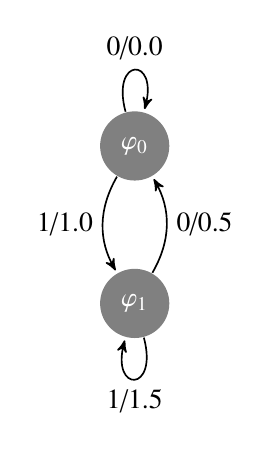
\begin{tikzpicture}[->,>=stealth',shorten >=1pt,auto,node distance=2.0cm,semithick]
  \tikzstyle{every state}=[fill=gray,draw=none,text=white]

  \node[state]         (B) {$\varphi_0$};

  \node[state]         (E) [below of=B]       {$\varphi_1$};

   \path     (B) edge [loop above] node {0/0.0} (B)
   			 (E) edge [bend right]  node[right] {0/0.5} (B)
             (B) edge[bend right]node[left]{1/1.0} (E)
        	 (E)  edge [loop below] node {1/1.5} (E);
\end{tikzpicture}

}
\caption{Finite state machine. }
\label{fig:FSM}
\end{figure}
The Trellis diagram for the FSM shown in Fig. \ref{fig:FSM} is given in Fig. \ref{fig:trellis}
\begin{figure}[h]
\centering
\resizebox{\columnwidth}{!}{
%\resizebox{\columnwidth}{!}{
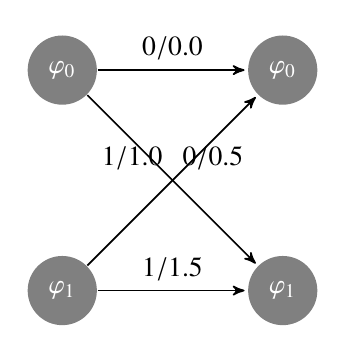
\begin{tikzpicture}[->,>=stealth',shorten >=1pt,auto,node distance=2.8cm,
                    semithick]
  \tikzstyle{every state}=[fill=gray,draw=none,text=white]

  \node[state] 			(A)                   {$\varphi_0$};
  \node[state]         (B) [ right of=A] {$\varphi_0$};
  \node[state]         (D) [below  of=A] {$\varphi_1$};
  \node[state]         (C) [below  of=B] {$\varphi_1$};
 
 
 \path (A) edge              node {$0/0.0$} (B)
            edge              node {$0/0.5$} (C)
        
            
        (D) edge              node {$1/1.5$} (C)
            
        
            edge              node {$1/1.0$} (B);
        


  
\end{tikzpicture}

}
\caption{Trellis Diagram. }
\label{fig:trellis}
\end{figure}

The multi-stage trellis diagram is shown in Fig. \ref{fig:multi-stage}.
\begin{figure}[h]
\centering
\resizebox{\columnwidth}{!}{
%\resizebox{\columnwidth}{!}{
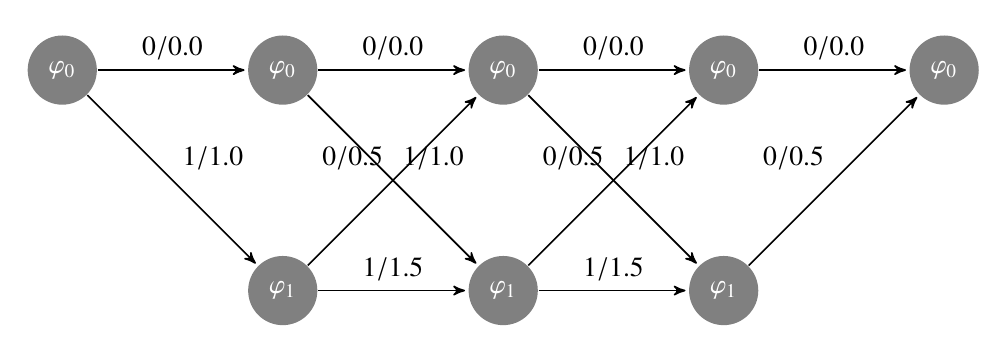
\begin{tikzpicture}[->,>=stealth',shorten >=1pt,auto,node distance=2.8cm,
                    semithick]
  \tikzstyle{every state}=[fill=gray,draw=none,text=white]

  \node[state] (A)                    {$\varphi_0$};
  \node[state]         (B) [right of=A] {$\varphi_0$};
  \node[state]         (C) [right of=B] {$\varphi_0$};
  \node[state]         (D) [right of=C] {$\varphi_0$};
  \node[state]         (E) [right of=D] {$\varphi_0$};
  \node[state]         (F) [below of=B] {$\varphi_1$};
  \node[state]         (G) [right of=F] {$\varphi_1$};    
  \node[state]         (H) [right of=G] {$\varphi_1$};   
  \path (A) edge              node {$0/0.0$} (B)
            edge              node {$1/1.0$} (F)
        (B) edge              node {$0/0.0$} (C)
            edge              node {$1/1.0$} (G)
        (C) edge              node {$0/0.0$} (D)
            edge              node {$1/1.0$} (H)
        (D) edge              node {$0/0.0$} (E)
        (F) edge              node {$0/0.5$} (C)
            edge              node {$1/1.5$} (G) 
        (G) edge              node {$0/0.5$} (D)
            edge              node {$1/1.5$} (H) 
        (H) edge              node {$0/0.5$} (E);
\end{tikzpicture}

}
\caption{Trellis Diagram. }
\label{fig:multi-stage}
\end{figure}

Suppose, we receive $r_k = [0.2,0.6,0.9,0.1]$ symbols at time instants $k=0,1,2,3$
\begin{itemize}
\item With Symbol-by-Symbol detection:
\begin{itemize}
\item Detection threshold  $= 0.5$.
\item Detected Symbols are $[0,1,1,0]$
\end{itemize}
\item ML detection/Minimum distance metric to be minimized
\begin{align}
\zeta_i = \sum_k \vert r_k - s_{k,i} \vert^2
\end{align}
Where, $i$ is over different transmit symbol vectors
\begin{equation}
\zeta_i = (r_0 - s_{0,i})^2 + (r_2 - s_{2,i})^2 \\ + (r_2 - s_{2,i})^2 + (r_3 - s_{3,i})^2
\label{eq:distance_metric}
\end{equation}
So, the branc metric at $k^{th}$ symbol period is
\begin{equation}
\zeta_{k,i} = (r_k - s_{k,i})^2
\end{equation}
Sum of these branch metrics to be minimized in MLSE.
\end{itemize}
The Trellis Diagram with branch metrics is shown in Fig. \ref{fig:branch_metric}.
\begin{figure}[h]
\centering
\resizebox{\columnwidth}{!}{
%\resizebox{\columnwidth}{!}{
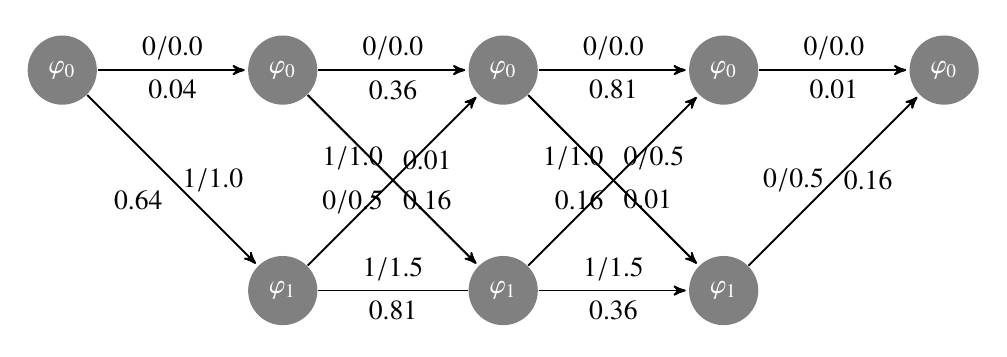
\begin{tikzpicture}[->,>=stealth',shorten >=1pt,auto,node distance=2.8cm,
                    semithick]
  \tikzstyle{every state}=[fill=gray,draw=none,text=white]

  \node[state] (A)                    {$\varphi_0$};
  \node[state]         (B) [right of=A] {$\varphi_0$};
  \node[state]         (C) [right of=B] {$\varphi_0$};
  \node[state]         (D) [right of=C] {$\varphi_0$};
  \node[state]         (E) [right of=D] {$\varphi_0$};
  \node[state]         (F) [below of=B] {$\varphi_1$};
  \node[state]         (G) [right of=F] {$\varphi_1$};    
  \node[state]         (H) [right of=G] {$\varphi_1$};   
  \draw (A)--node[above] {$0/0.0$}(B);
  \draw (A)--node[below] {$0.04$}(B);
  \draw (A)--node[right] {$1/1.0$}(F);
  \draw (A)--node[below left] {$0.64$}(F);
  \draw (B)--node[above] {$0/0.0$}(C);
  \draw (B)--node[below] {$0.36$}(C);
  \draw (C)--node[above] {$0/0.0$}(D);
  \draw (C)--node[below] {$0.81$}(D);
  \draw (D)--node[above] {$0/0.0$}(E);
  \draw (D)--node[below] {$0.01$}(E);
  \draw (B)--node[above left] {$1/1.0$}(G);
  \draw (B)--node[above right] {$0.01$}(G);
  \draw (F)--node[below left] {$0/0.5$}(C);
  \draw (F)--node[below right] {$0.16$}(C);
  \draw (C)--node[above left] {$1/1.0$}(H);
  \draw (C)--node[below right] {$0.01$}(H);
  \draw (G)--node[above right] {$0/0.5$}(D);
  \draw (G)--node[below left] {$0.16$}(D);
  \draw (H)--node[left] {$0/0.5$}(E);
  \draw (H)--node[right] {$0.16$}(E);
  \draw (F)--node[above] {$1/1.5$}(G) --node[above] {$1/1.5$}(H);
  \draw (F)--node[below] {$0.81$}(G) --node[below] {$0.36$}(H);
\end{tikzpicture}

}
\caption{Trellis Diagram with branch metrics. }
\label{fig:branch_metric}
\end{figure}
The shortest path using Viterbi Algorithm (VA) is shown in Fig. \ref{fig:shortest_path}.
\begin{figure}[h]
\centering
\resizebox{\columnwidth}{!}{
%\resizebox{\columnwidth}{!}{
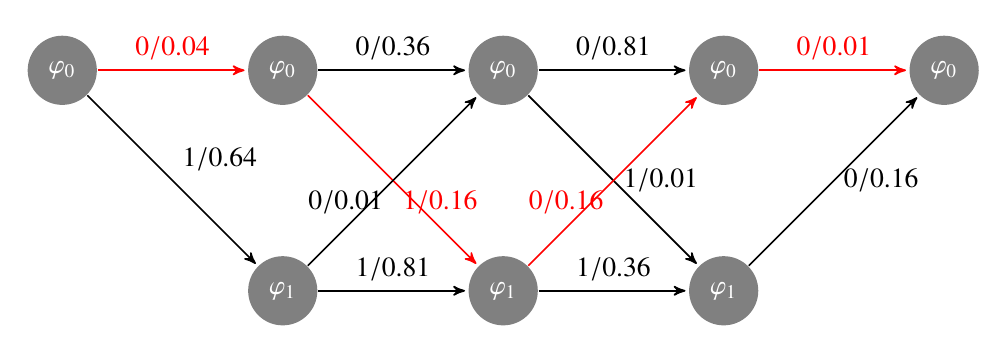
\begin{tikzpicture}[->,>=stealth',shorten >=1pt,auto,node distance=2.8cm,
                    semithick]
  \tikzstyle{every state}=[fill=gray,draw=none,text=white]

  \node[state] (A)                    {$\varphi_0$};
  \node[state]         (B) [right of=A] {$\varphi_0$};
  \node[state]         (C) [right of=B] {$\varphi_0$};
  \node[state]         (D) [right of=C] {$\varphi_0$};
  \node[state]         (E) [right of=D] {$\varphi_0$};
  \node[state]         (F) [below of=B] {$\varphi_1$};
  \node[state]         (G) [right of=F] {$\varphi_1$};    
  \node[state]         (H) [right of=G] {$\varphi_1$};   
  \path (A) edge [color=red]              node {$0/0.04$} (B)
            edge              node {$1/0.64$} (F)
        (B) edge              node {$0/0.36$} (C)
            edge [color=red]             node[below right] {$1/0.16$} (G)
        (C) edge              node {$0/0.81$} (D)
            edge              node[right] {$1/0.01$} (H)
        (D) edge [color=red]             node {$0/0.01$} (E)
        (F) edge               node[below left] {$0/0.01$} (C)
            edge              node {$1/0.81$} (G) 
        (G) edge[color=red]              node[below left] {$0/0.16$} (D)
            edge              node {$1/0.36$} (H) 
        (H) edge              node[right] {$0/0.16$} (E);
\end{tikzpicture}

}
\caption{Trellis Diagram with branch metrics. }
\label{fig:shortest_path}
\end{figure}
The symbol-by-symbol detection gives $[0,1,1,0]$ and
Maximum Likelihood sequence estimation (Via VA) gives $[0,1,0,0]$.
\subsubsection{Trellis structure in Code}
There are total $M^{L-1}$ states in the trellis. The complexity of viterbi algorithm increases with the length of the channel filter.
Suppose $L=3$ and number of states in trellis $64$. The total number of outpus from the trellis is
\begin{align}
trellis\_out\_size &= 64*M 
\end{align} 
$Trellis\_in\_struct$ and $Trellis\_out\_struct$ 

The ML sequence estimator structure using viterbi algorithm  \cite{viterbi} is shown in \cite{MLSE} and \cite{Proakis}.
To estimate a sequence of length $m$, the receiver complexity is $M^m$ symbols for finding the most likely sequence among $M^m$ sequences. However, this complexity can be reduced from $M^m$ to $M^{L-1}$, where $L$ is the number of states in trellis used for viterbi Algorithm ($L < m$).

The number of the states in the trellis increaes exponetially ($M^{L-1}$) with lenghth of the channel impulse response ($L$). Since the bandwidth requirement is $250$ Khz, the length of the impulse response is suficient to assume as $3$ and implemneted the viterbi algorithm with $64$ states.

\section{Channel Estimation}
The MLSE via Viterbi Algorithm needs the channel state information for finding the shortest path. The channel can be estimated using Fast Fourier transforms for a sequence of pilot symbols.

We have used $10$ pilot symbols in the code for the estimation of channel. The observed symbols at the receiver  for the pilot symbols is given by
\begin{equation}
\textbf{r}_{p} = \textbf{h}*\textbf{x}_{p} + \textbf{n}_{p}
\end{equation}

The steps for channel estimation is given below 
\begin{itemize}
\item Make $\textbf{r}_{p}$ into a circular convolution of \textbf{h} and $\textbf{x}_{p}$ by removing  last $L-1$ symbols from $\textbf{r}_{p}$ to add them to the first $L-1$ symbols .
\item Find 
\begin{align}
Y = fft \left(\textbf{r}_{p}\right) \quad X = fft \left(\textbf{x}_{p}\right) 
\end{align}
\item Find first three taps of $h_{est}$ from
\begin{align}
h_{est} = ifft\left(\frac{Y}{X}\right)
\end{align}
 \end{itemize}
 
The second method for channel estimation based on Toeplitz matrix method with pilot symbols is given below
\begin{itemize}
\item Construct a toeplitz matrix $X$  with pilot symbols $x_p$.
\item 
\begin{align}
h_est = \left(X^{*}X\right)^{-1}X^{*}y_p
\end{align}
\end{itemize}

\section{Zero Forcing Equalizer and MMSE Equalizer}
The Zero-Forcing Equalizer and MMSE are implemente using Toeplitz matrices \cite{eq}.
\subsection{Zero Forcing Equalizer}
\begin{itemize}
\item Construct a toeplitz matrix $H$  with estimated channel $h_{est}$.
\item 
\begin{align}
x_{hat} = \left(H^{*}H\right)^{-1}H^{*}y
\end{align}
\end{itemize}
\subsection{MMSE Equalizer}
\begin{itemize}
\item Construct a toeplitz matrix $H$  with estimated channel $h_{est}$.
\item 
\begin{align}
x_{hat} = \left(H^{*}H + \frac{I}{SNR} \right)^{-1}H^{*}y
\end{align}
Where, $I$ is an identity matrix and $SNR$ is the signal-to-noise ratio.
\end{itemize}

%\section{Simulation results}
%We have trained for $100$ $8-PSK$ symbols ($30$ Frames ($1 Frame = 40 bytes$)) for $15$ iterations and in Fig.\ref{fig:MMSE} and Fig. \ref{fig:DFE}, the convergence of cost function (Mean Square Error (MSE)) w.r.to the number of iterations for both MMSE and DFE equalizers are shown.
%%\subsection{Plots}
%\begin{figure}[t]
%\begin{center}
%\includegraphics[width=\columnwidth]{./figs/Cost Function MMSE.eps}
%\end{center}
%\caption{Mean Sqaure Error Vs Iterations for MMSE}
%\label{fig:MMSE}
%\end{figure}
%
%\begin{figure}[t]
%\begin{center}
%\includegraphics[width=\columnwidth]{./figs/Cost Function DFE.eps}
%\end{center}
%\caption{Mean Sqaure Error Vs Iterations for MMSE}
%\label{fig:DFE}
%\end{figure}
%
%Table \ref{table:comparisions} compares the different equalizers explained in previous sections.
%
%\begin{table}[b]
%\caption{Comparision of different Equalizers}
%\begin{center}
%\begin{tabular}{|c|c|c|c|}
%\hline
%\textbf{Equalizer}& \textbf{Frames} & \text{Time} & \textbf{Complexity}\\
%    \hline
%    $MMSE$ & 60 & 120 ms & Medium\\ %\quad \cite{bitnodes} \\
%    \hline
%    $DFE$ & 120 & 240 ms & Medium\\ %\quad \cite{bitnodes}  \\
%    \hline
%    $MLSE$ & $-$ & $-$ & High \\
%		\hline
%	
%\end{tabular}
%\label{table:comparisions}
%\end{center}
%\end{table}
%
%
%Fig.\ref{fig:ser} shows the SER curve ($\frac{E_b}{N_0} vs P_{e}$).
%\begin{figure}[!t]
%\begin{center}
%\includegraphics[width=\columnwidth]{./figs/Equalizers_1.eps}
%\end{center}
%\caption{Symbol Error Rate}
%\label{fig:ser}
%\end{figure}
%
%
\bibliography{IEEEabrv,equalization.bib}
\end{document}
